% =====================================================================
%  Group-Fair Stochastic Gradient Descent via Masked Optimal Transport
%  ICASSP submission -- 4 pages + 1 page references
%
%  Compile:  pdflatex main ; pdflatex main
%  Replace the local stand-in spconf.sty with the official ICASSP one
%  before submitting. Nothing in this file needs to change.
%
%  Markers you should sweep before submission:
%     %%FILLIN   -- a number or description only you can supply
%     %%CHECK    -- a claim worth re-reading against the code
% =====================================================================
\documentclass{article}
\usepackage{spconf,amsmath,amssymb,amsthm,graphicx,booktabs,multirow}
\usepackage{algorithm}
\usepackage{algpseudocode}
\usepackage[usenames,dvipsnames]{xcolor}
\usepackage{url}
\usepackage{tikz}
\usetikzlibrary{positioning,arrows.meta,fit,backgrounds}

% ---------------------------------------------------------------- macros
\newtheorem{theorem}{Theorem}
\newtheorem{lemma}[theorem]{Lemma}
\newtheorem{proposition}[theorem]{Proposition}
\newtheorem{corollary}[theorem]{Corollary}
\theoremstyle{definition}
\newtheorem{assumption}[theorem]{Assumption}
\newtheorem{remark}[theorem]{Remark}

\newcommand{\R}{\mathbb{R}}
\newcommand{\E}{\mathbb{E}}
\newcommand{\PP}{\mathbb{P}}
\newcommand{\Nn}[1]{[#1]}
\newcommand{\simplex}[1]{\Delta^{#1-1}}
\newcommand{\CVaR}{\mathrm{CVaR}}
\newcommand{\KL}{\mathrm{KL}}
\newcommand{\Proj}{\Pi_{\mathcal{C}}}
\newcommand{\avot}{\textsf{GAVOT}}
\newcommand{\avotcvar}{\textsf{GAVOT+CVaR}}
\DeclareMathOperator*{\argmin}{arg\,min}
\DeclareMathOperator*{\argmax}{arg\,max}

\newcommand{\best}[1]{\textbf{#1}}

% ---------------------------------------------------------------- title
\title{Group-Fair Stochastic Gradient Descent \\ via Masked Optimal Transport}

\name{Herlock (SeyedAbolfazl) Rahimi \qquad Dionysis Kalogerias%
\thanks{This work is supported by NSF under Grant 2242215.}}
\address{Department of Electrical and Computer Engineering, Yale University, New Haven, CT, USA\\
\texttt{\{herlock.rahimi, dionysis.kalogerias\}@yale.edu}}

\newlabel{sec:setup}{{2}{2}{}{section.2}{}}
\newlabel{eq:target}{{1}{2}{}{equation.1}{}}
\newlabel{ass:std}{{1}{2}{}{theorem.1}{}}
\newlabel{prop:surrogate}{{2}{2}{}{theorem.2}{}}
\newlabel{sec:cvar}{{4}{4}{}{section.4}{}}
\newlabel{sec:exp}{{5}{4}{}{section.5}{}}
\bibcite{buolamwini2018gender}{1}
\bibcite{hashimoto2018repeated}{2}
\bibcite{sagawa2020dro}{3}
\bibcite{mohri2019agnostic}{4}
\bibcite{li2020fair}{5}
\bibcite{rahimi2025fedavot}{6}
\bibcite{rahimi2025agnostic}{7}
\bibcite{wang2020objective}{8}
\bibcite{cho2022biased}{9}
\bibcite{mcmahan2017fedavg}{10}
\bibcite{agarwal2018reductions}{11}
\bibcite{cotter2019twoplayer}{12}
\bibcite{chamon2020pacc}{13}
\bibcite{chamon2023nonconvex}{14}
\bibcite{rahimi2026exactpenalty}{15}
\bibcite{rizk2021importance}{16}
\bibcite{katharopoulos2018not}{17}
\bibcite{sinkhorn1967}{18}
\bibcite{cuturi2013}{19}
\bibcite{peyre2019}{20}
\bibcite{gietl2013ipfp}{21}
\bibcite{csiszar1975}{22}
\bibcite{hall1935}{23}
\bibcite{fordfulkerson1956}{24}
\bibcite{villani2009}{25}
\bibcite{rockafellar2000cvar}{26}
\bibcite{curi2020adaptive}{27}
\bibcite{levy2020large}{28}
\bibcite{namkoong2017variance}{29}
\bibcite{nemirovski2009}{30}
\bibcite{li2020fedprox}{31}
\bibcite{karimireddy2020scaffold}{32}
\bibcite{uci_adult}{33}
\bibcite{rothe2018imdbwiki}{34}
\bibcite{theodoropoulos2024restricted}{35}
\title{Sec. 3 Proposed Approach}
\name{}\address{}
\begin{document}\ninept\maketitle
% =====================================================================
%  Section 3: Proposed Approach  (replaces "Alignment by Masked Optimal
%  Transport" in main.tex; all labels kept).  Structure follows FedAVOT
%  Sec. 2-3: coupling, feasibility (Hall/flow), Sinkhorn, algorithm,
%  unbiasedness, second moment, rate, infeasible regime.
% =====================================================================
\section{Proposed Approach: Alignment by Masked Optimal Transport}
\label{sec:gavot}
% =====================================================================

\noindent\textbf{Weights as a coupling.}
Let $Y[i,j]\ge 0$ be the weight assigned to group $i$ when the active set is
$A_j$, with $Y[i,j]=0$ for $i\notin A_j$, and let $T[i,j]\triangleq q_jY[i,j]$
be the joint mass carried from composition $j$ to group $i$. Requiring that
the weights be a probability vector on each realized composition, and that
each group receive in expectation the mass $p$ assigns it, is the
\emph{masked optimal transport} (MOT) feasibility problem of
\cite{rahimi2025fedavot},
\begin{equation}
T\mathbf{1}_M=p,\qquad \mathbf{1}_N^\top T=q,\qquad T\ge 0,
\qquad \mathrm{supp}(T)\subseteq E,
\label{eq:mot}
\end{equation}
with mask $E=\{(i,j): i\in A_j\}$ encoding that a group absent from the batch
cannot be weighted. Unlike classical transport
\cite{villani2009,peyre2019} there is no cost to minimize: any coupling
respecting \eqref{eq:mot} serves, and \eqref{eq:mot} is the Kantorovich
problem with the indicator cost $C[i,j]=\infty$ off $E$. Fig.~\ref{fig:mask}
is the picture.

\begin{figure}[t]
\centering
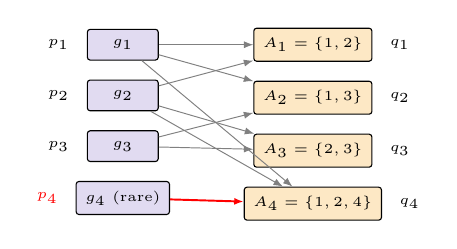
\begin{tikzpicture}[
   node distance=2.4mm,
   grp/.style={draw,rounded corners=1pt,minimum width=9mm,minimum height=3.9mm,font=\tiny,fill=Periwinkle!20},
   atm/.style={draw,rounded corners=1pt,minimum width=13mm,minimum height=3.9mm,font=\tiny,fill=YellowOrange!20},
   e/.style={-{Latex[length=1.2mm]},gray,line width=.35pt},
   lbl/.style={font=\tiny\itshape}
]
\node[grp] (g1) {$g_1$};
\node[grp,below=of g1] (g2) {$g_2$};
\node[grp,below=of g2] (g3) {$g_3$};
\node[grp,below=of g3] (g4) {$g_4$ \tiny(rare)};

\node[atm,right=12mm of g1] (a1) {$A_1=\{1,2\}$};
\node[atm,below=of a1] (a2) {$A_2=\{1,3\}$};
\node[atm,below=of a2] (a3) {$A_3=\{2,3\}$};
\node[atm,below=of a3] (a4) {$A_4=\{1,2,4\}$};

\draw[e] (g1)--(a1); \draw[e] (g2)--(a1);
\draw[e] (g1)--(a2); \draw[e] (g3)--(a2);
\draw[e] (g2)--(a3); \draw[e] (g3)--(a3);
\draw[e] (g1)--(a4); \draw[e] (g2)--(a4); \draw[e,Red,line width=.7pt] (g4)--(a4);

\node[lbl,left=1mm of g1] {$p_1$};
\node[lbl,left=1mm of g2] {$p_2$};
\node[lbl,left=1mm of g3] {$p_3$};
\node[lbl,left=1mm of g4,Red] {$p_4$};
\node[lbl,right=1mm of a1] {$q_1$};
\node[lbl,right=1mm of a2] {$q_2$};
\node[lbl,right=1mm of a3] {$q_3$};
\node[lbl,right=1mm of a4] {$q_4$};
\end{tikzpicture}
\caption{The mask $E$. Batch compositions carry the mass $q$ they occur with;
groups must receive the mass $p$ the objective assigns them. Group $4$ is
reachable only through $A_4$, so exact alignment requires $p_4\le q_4$: the
Hall condition of Thm.~\ref{thm:feas} read on the singleton $I=\{4\}$. Shrinking
the batch deletes $A_4$ from the support and makes $p_4$ unreachable.}
\label{fig:mask}
\end{figure}

\noindent\textbf{When alignment is possible.}
Existence of a coupling is a supply--demand question on the bipartite graph
$E$, and is settled by flow duality.

\begin{theorem}[Feasibility, {\cite[Thm.~1]{rahimi2025fedavot}}]
\label{thm:feas}
For $I\subseteq\Nn{N}$ let $\mathcal{N}(I)=\{j:\exists\,i\in I,\ (i,j)\in E\}$
and $\mathcal{S}(I)=\{j: A_j\subseteq I\}$. Problem \eqref{eq:mot} is feasible
if and only if
\begin{equation}
\sum_{j\in\mathcal{S}(I)}q_j\;\le\;\sum_{i\in I}p_i\;\le\;\sum_{j\in\mathcal{N}(I)}q_j
\qquad\forall\,I\subseteq\Nn{N}.
\label{eq:hall}
\end{equation}
\end{theorem}
Proofs are in the appendix. Read on singletons, \eqref{eq:hall} becomes a
statement one can act on before training starts.

\begin{corollary}[Coverage law and severity]
\label{cor:batchsize}
Feasibility of \eqref{eq:mot} requires $\PP[A^t=\{i\}]\le p_i\le r_i$ for every
$i$, with $r_i=\PP[i\in A^t]$ the observation rate of Sec.~\ref{sec:setup}.
Writing
\begin{equation}
\nu\;\triangleq\!\!\sum_{i\,:\,p_i>r_i}\!\! p_i
\label{eq:batchlaw}
\end{equation}
for the \emph{infeasible mass}, $\nu=0$ iff the upper constraints hold.
Under i.i.d.\ sampling of $b$ examples the upper constraint reads
$b\ge\log(1-p_i)/\log(1-\pi_i)$; under $K$-of-$N$ uniform group sampling it
reads $p_i\le K/N$.
\end{corollary}
\noindent\textbf{Severity.}
Importance may not exceed observation rate: a rare group is reachable only
if the batch is large enough to contain it often enough. The infeasible mass
$\nu$ is the axis we sweep: at $\nu=0$ exact alignment is available, and as
$\nu$ grows more of $p$ sits outside the set of row marginals the mask can
reach. A \emph{feasible} and an \emph{infeasible} regime are two points on
this continuum, and Sec.~\ref{sec:exp} sweeps it instead.

\noindent\textbf{Computing the plan.}
Given feasibility, a coupling is obtained by iterative proportional fitting
(Sinkhorn scaling) on the masked support
\cite{sinkhorn1967,cuturi2013,peyre2019}: starting from any $T^{(0)}>0$ on
$E$ with $\mathbf{1}^\top T^{(0)}=q$, alternate
\begin{equation}
T\leftarrow\mathrm{diag}\big(p\oslash T\mathbf{1}\big)\,T,\qquad
T\leftarrow T\,\mathrm{diag}\big(q\oslash T^\top\mathbf{1}\big)
\label{eq:ipfp}
\end{equation}
until $\|T\mathbf{1}-p\|_1\le\varepsilon$. Each sweep costs $O(|E|)$ with
$|E|\le NM$ and $M$ the number of \emph{realized} compositions rather than
$2^N$; the plan is computed once, offline, and the training loop adds one
lookup and one multiply per group per step. Under \eqref{eq:hall} the
iteration converges to a solution of \eqref{eq:mot}
\cite{sinkhorn1967,csiszar1975}, being block-coordinate ascent on the dual of
the entropic problem $\min\{\sum_E T\log T:\ T\mathbf{1}=p,\ \mathbf{1}^\top T=q\}$.
Since $\mathbf{1}_N^\top T=q$ and $Y=T\mathrm{diag}(q)^{-1}$, every column
$Y[\cdot,j]$ is a probability vector on $A_j$, the property each bound below
uses. Algorithm~\ref{alg:gavot} is the resulting method; $\gamma=1$ is the
risk-neutral rule analyzed here and $\gamma<1$ the risk-averse layer of
Sec.~\ref{sec:cvar}.

\begin{algorithm}[t]
\caption{\avot{}: group-fair SGD by masked transport}
\label{alg:gavot}
\begin{algorithmic}[1]
\Require target $p$, composition law $(q,\{A_j\},E)$, step $\eta$, horizon $T$,
 CVaR parameters $(\alpha,\gamma)$ with $\gamma=1$ for the risk-neutral method
\State $(T,Y)\leftarrow$ Sinkhorn scaling for $(p,q,E)$ \Comment{offline, once}
\State $\theta^0\in\mathcal{C}$, $\ t^0\in\R$
\For{$t=1,\dots,T$}
  \State draw batch $B^t$; set $A^t$, let $j(t)$ be s.t.\ $A_{j(t)}=A^t$
  \State $g^t_i \leftarrow$ stochastic subgradient of $f_i$ from $B^t\cap$ group $i$
  \State $w^t_i \leftarrow Y[i,j(t)]\big(\gamma+\tfrac{1-\gamma}{\alpha}\mathbf{1}\{\hat f^t_i>t^{t-1}\}\big)$
  \State $\theta^{t}\leftarrow\Proj\big(\theta^{t-1}-\eta\sum_{i\in A^t}w^t_i\,g^t_i\big)$
  \State $t^{t}\leftarrow t^{t-1}-\eta(1-\gamma)\big(1-\tfrac{1}{\alpha}\sum_{i\in A^t}Y[i,j(t)]\mathbf{1}\{\hat f^t_i>t^{t-1}\}\big)$
\EndFor
\Ensure $\bar\theta_T=\frac{1}{T}\sum_{t=1}^{T}\theta^t$
\end{algorithmic}
\end{algorithm}

\noindent\textbf{Analysis.}
Everything rests on one identity, \cite[Lem.~1]{rahimi2025fedavot} moved from
model averaging to gradient averaging. Let $g_i(\theta)$ be the stochastic
subgradient of $f_i$ computed from $B^t\cap$ group $i$ and
$\hat g(\theta)=\sum_{i\in A^t}Y[i,j(t)]\,g_i(\theta)$ the transport-weighted
batch subgradient of Algorithm~\ref{alg:gavot}. Transport removes bias; it is
not a variance reduction device.

\begin{lemma}[Unbiasedness]
\label{lem:unbiased}
Let $T$ satisfy \eqref{eq:mot}. Then $\E[\hat g(\theta)\mid\theta]\in\partial F_p(\theta)$
for every $\theta\in\mathcal{C}$.
\end{lemma}
\begin{proof}
Conditionally on $A^t=A_j$, $\E[g_i(\theta)]\in\partial f_i(\theta)$ for
$i\in A_j$. Averaging over $A^t\sim q$,
$\E[\hat g]=\sum_j q_j\sum_{i\in A_j}Y[i,j]\,\partial f_i(\theta)
=\sum_i\big(\sum_j T[i,j]\big)\partial f_i(\theta)=\sum_i p_i\,\partial f_i(\theta)$,
the row-marginal constraint being used in the last step.
\end{proof}

\begin{lemma}[Second moment, free of coverage]
\label{lem:variance}
$\E\|\hat g(\theta)\|^2\le G^2$ for every $\theta\in\mathcal{C}$, with no
dependence on $|A^t|$ or on $N$.
\end{lemma}
\begin{proof}
$Y[\cdot,j]$ is a probability vector on $A_j$, so
$\|\sum_i Y[i,j]g_i\|^2\le\sum_i Y[i,j]\|g_i\|^2$ by convexity of
$\|\cdot\|^2$; take expectations and use $\sum_j T[i,j]=p_i$:
$\E\|\hat g\|^2\le\sum_i p_i\,\E\|g_i\|^2\le G^2$.
\end{proof}

\begin{theorem}[Rate]
\label{thm:rate}
Under Assumption~\ref{ass:std}, if \eqref{eq:mot} is feasible then
Algorithm~\ref{alg:gavot} with $\gamma=1$ and $\eta=D/(G\sqrt{T})$ satisfies
\begin{equation}
\E\big[F_p(\bar\theta_T)\big]-F_p(\theta^\star)\;\le\;\frac{DG}{\sqrt{T}} .
\label{eq:rate}
\end{equation}
\end{theorem}
The constant in \eqref{eq:rate} is that of full-participation SGD and is
independent of how many groups appear in a batch: a composition covering two
groups yields the same bound as one covering all $N$, though with larger
realized variance. The proof uses only the two lemmas and never refers to
$|A^t|$, which is why the rate of \cite{rahimi2025fedavot} transfers verbatim
from aggregation of models to aggregation of gradients.

\noindent\textbf{Outside the feasible region.}
When \eqref{eq:hall} fails, \eqref{eq:mot} has no solution and the iteration
\eqref{eq:ipfp} does not diverge: its iterates accumulate at the coupling
whose row marginal $\hat p\triangleq T\mathbf{1}$ is the KL-closest to $p$
over the reachable polytope
$\mathcal{R}(q,E)=\{T\mathbf{1}:\ T\ge 0,\ \mathbf{1}^\top T=q,\ \mathrm{supp}(T)\subseteq E\}$
\cite{csiszar1975,gietl2013ipfp,peyre2019}. The column marginal is met
exactly, so Lemmas~\ref{lem:unbiased} and~\ref{lem:variance} hold with $p$
replaced by $\hat p$: Algorithm~\ref{alg:gavot} is then unbiased SGD on the
surrogate $F_{\hat p}$, the closest objective the sampler can reach, and the
loss on \eqref{eq:target} is a bias of exactly the shape of
Proposition~\ref{prop:surrogate}. On singletons $\hat p_i\le r_i$, so the
groups with $p_i>r_i$ are truncated at their observation rate and their
missing mass, $\nu$ up to renormalization, is redistributed.

\begin{theorem}[Infeasible regime]
\label{thm:infeasible}
Let $\hat p$ be the row marginal of the Sinkhorn limit,
$\theta^\dagger\in\argmin_{\mathcal{C}}F_{\hat p}$, and write
$\Phi(w)\triangleq F_p\big(\argmin_{\mathcal{C}} F_w\big)$ for the $p$-risk of
the minimizer of the $w$-weighted risk. Then
\begin{equation}
\E\big[F_p(\bar\theta_T)\big]-F_p(\theta^\star)
\;=\;\underbrace{\Phi(\hat p)-\Phi(p)}_{\text{alignment floor}}
\;+\;\underbrace{\varepsilon_T(\hat p)}_{\text{optimization residual}} ,
\label{eq:infeasible}
\end{equation}
where $\varepsilon_T(\hat p)\triangleq\E F_p(\bar\theta_T)-F_p(\theta^\dagger)$
satisfies $\E F_{\hat p}(\bar\theta_T)-F_{\hat p}(\theta^\dagger)\le DG/\sqrt{T}$
and $\varepsilon_T(\hat p)\to 0$ whenever $\bar\theta_T\to\theta^\dagger$.
Group-blind averaging obeys \eqref{eq:infeasible} with $\tilde p$ in place of
$\hat p$. Writing $\Delta_{\mathrm{floor}}\triangleq\Phi(\tilde p)-\Phi(\hat p)$
for the \emph{alignment gain}, transport improves on group-blind averaging
exactly when $\Delta_{\mathrm{floor}}>\varepsilon_T(\hat p)-\varepsilon_T(\tilde p)$,
and every floor is bounded by $\Phi(w)-\Phi(p)\le 2M\|p-w\|_1$.
\end{theorem}
Theorem~\ref{thm:infeasible} replaces the usual bias \emph{bound}
\cite{rahimi2025fedavot} by an exact \emph{decomposition}, both terms of which
are available before training: $\hat p$ and $\tilde p$ from $(p,q,E)$, and
$\Phi$ exactly on instances with a closed-form or convex frontier. The gain is
fixed by the instance and decides the sign of the comparison; the residual is
paid by the estimator and, as Sec.~\ref{sec:exp} shows, is a stepsize
artifact. The $\ell_1$ bound is the weaker object and we report both, because
it turns out too loose to discriminate.

\end{document}
